\section{Data Processing Pipeline}

WhiteTiger transforms heterogeneous human-teleoperated robot operation records into a consistent dataset for large-scale policy training. Fig.~\ref{fig:data-processing-pipeline} summarizes the conversion from platform-specific HDF5 trajectories to model-ready LeRobot v2.1 records through validation, filtering, metadata standardization, embodiment-schema alignment, and format conversion. The pipeline preserves embodiment-specific control semantics, rejects invalid or task-inconsistent trajectories, and exposes a unified interface for robot learning systems.

\begin{figure}[t]
\centering
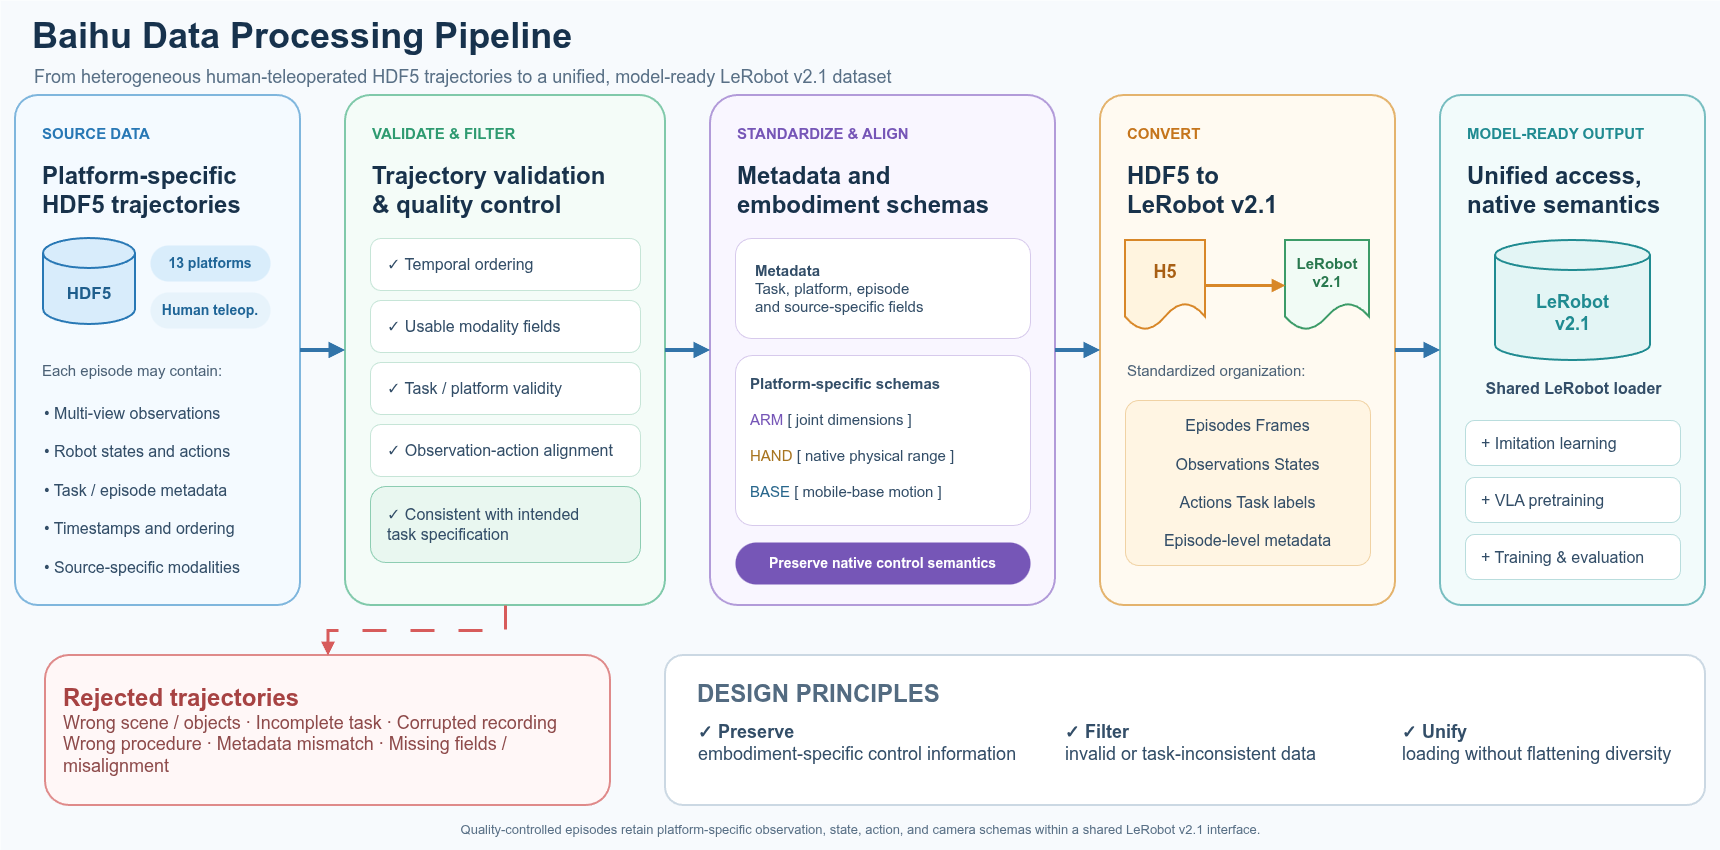
\includegraphics[width=\textwidth]{figures/pipeline2.png}
\caption{Data processing pipeline of WhiteTiger. Platform-specific HDF5 trajectories collected through human teleoperation are validated and filtered, standardized with task and platform metadata, aligned with embodiment-specific state and action schemas, and converted into LeRobot v2.1. The pipeline rejects trajectories with invalid scene setup, incomplete execution, corrupted recordings, metadata mismatch, missing modality fields, or observation-action misalignment, while preserving native control semantics for downstream imitation learning, vision-language-action adaptation, event-aware learning, and benchmark evaluation.}
\label{fig:data-processing-pipeline}
\end{figure}

\subsection{HDF5 ingestion and trajectory validation}

Raw WhiteTiger trajectories are organized as HDF5 records. Each record is associated with a robot platform, task identity, episode identity, and available modality fields. Source trajectories may contain visual observations, proprioceptive states, actions, task annotations, timestamps, and episode-level metadata, depending on platform and task setup.

Validation is required before trajectories enter the released training corpus. The pipeline checks temporal ordering, usable modality fields, task metadata consistency, platform metadata validity, and observation-action alignment. This stage removes incomplete, corrupted, or unusable trajectories that would otherwise create incorrect supervision during model training.

\subsection{Quality control and metadata standardization}

WhiteTiger uses a multi-stage quality-control workflow covering acquisition, monitoring, upload, validation, cleaning, review, and final delivery. At billion-frame scale, a small invalid fraction can correspond to a large amount of corrupted supervision. Quality control therefore constrains noise introduced by heterogeneous platforms while retaining the embodiment and interaction diversity required for foundation-model adaptation.

A trajectory is retained only when it satisfies the requester-defined task specification. Removal cases include incorrect scene setup, incorrect objects or tools, wrong manipulation procedure, incomplete execution, corrupted recording, missing modality fields, inconsistent task metadata, and observation-action misalignment. Failed or task-inconsistent demonstrations are not intentionally preserved as training examples in the released corpus.

Task and episode metadata are standardized for dataset analysis and model conditioning. Each episode is associated with task information, platform metadata, and source-specific fields when available. Manual task annotations provided at collection-request time supply language or semantic conditioning signals for vision-language-action policies. Metadata standardization checks that the recorded trajectory remains consistent with the intended task description.

\subsection{State and action schema alignment}

State and action schemas differ across robot platforms. Joint layouts, gripper structures, dexterous-hand dimensions, mobile-base commands, control frequencies, and action semantics are platform-dependent. WhiteTiger preserves schemas that identify arm joints, grippers, hands, bases, and other controllable components within each platform.

Schema alignment enables unified dataset loading without erasing native control spaces. For the planned offline evaluation, Joint MSE will use only joint-related action dimensions, while ALL MSE will use the complete action vector for each platform. End-effector values are stored according to the physical travel range of each platform. WhiteTiger does not impose a universal gripper or hand scale across robots, preserving the action values used by the original controllers.

\subsection{HDF5-to-LeRobot v2.1 conversion}

After validation and schema alignment, source HDF5 records are converted into LeRobot v2.1. The conversion standardizes episode and frame organization, synchronized visual observations, robot states, actions, human-provided task annotations, event or keyframe annotations when available, and episode-level metadata. HDF5 remains the source trajectory container, while LeRobot v2.1 provides the training interface for dataset loading, episode management, and downstream evaluation.

WhiteTiger does not force every platform into an identical observation or action vector. Each robot retains its modality-specific state, action, and camera schema within the shared LeRobot v2.1 interface. This design supports consistent data access across platforms while preserving the physical control semantics required for cross-embodiment policy learning.

\section{Planned Benchmark Evaluations}

\subsection{Planned offline open-loop zero-shot evaluation}

We plan to conduct an offline open-loop zero-shot action-prediction evaluation to assess whether WhiteTiger fine-tuning improves transfer to robot demonstration datasets that are external to, and excluded from, the WhiteTiger training corpus. The planned comparison will use the same foundation-model architecture for a pretrained baseline and a WhiteTiger-fine-tuned model. Neither model will be adapted on the external evaluation datasets. Zero-shot will therefore refer to dataset-level transfer from WhiteTiger training to separately collected evaluation trajectories.

Under recorded observations, each model will predict robot actions that will be compared with the corresponding human-teleoperation actions. The same held-out trajectories will be used for both models to form paired comparisons. The evaluation scope, trajectory-sampling rules, prediction horizon, and aggregation procedure will be fixed before the results are analyzed.

The planned primary metric is normalized full-action MSE, computed over the complete platform-specific action vector. A joint-only normalized MSE will provide an auxiliary diagnostic that excludes gripper or dexterous-hand actuation dimensions. Results are planned to be reported at task, platform, and overall levels, together with sampling variability or confidence intervals where appropriate. Because this evaluation has not yet been completed, the current paper does not report quantitative offline zero-shot results or make performance-improvement claims from this protocol.

\subsection{Planned real-world evaluation of event-guided value learning}

The planned offline evaluation will assess the dense-trajectory function of WhiteTiger for foundation-model adaptation and cross-dataset action prediction. Event- and keyframe-level annotations target a separate question: whether explicit task-progress supervision improves closed-loop execution. A planned real-world protocol will compare policies trained with and without event-derived value supervision.

Both policies will start from the same supervised fine-tuned model and will be evaluated on the same real-robot tasks under randomized initial configurations. The baseline policy will use dense trajectory supervision without event-derived value learning. The event-guided policy will use WhiteTiger event and keyframe annotations to construct task-progress supervision from subgoal and event completion. This design is intended to isolate the contribution of temporal annotations under real execution.

The planned evaluation will cover representative robot embodiments and manipulation tasks. Execution success rate will be the primary metric. Event completion rate, failure-stage distribution, and time to completion will provide diagnostic measures. Until these experiments are completed, event-guided value learning remains a planned evaluation direction rather than a demonstrated performance claim.

\subsection{Future benchmark extensions}

Natural extensions include data-scaling curves for policy scaling-law analysis, held-out-platform evaluation for cross-embodiment generalization, closed-loop simulation evaluation, additional policy families, and real-world rollout success-rate experiments. These extensions will complement the planned offline open-loop zero-shot evaluation by testing generalization under broader model and execution settings.
